\documentclass{article}
\usepackage[final]{neurips_2019}
\usepackage[utf8]{inputenc} % allow utf-8 input
\usepackage[T1]{fontenc}    % use 8-bit T1 fonts
\usepackage{hyperref}       % hyperlinks
\usepackage{url}            % simple URL typesetting
\usepackage{booktabs}       % professional-quality tables
\usepackage{amsfonts}       % blackboard math symbols
\usepackage{nicefrac}       % compact symbols for 1/2, etc.
\usepackage{microtype}      % microtypography
\usepackage{bbm}

\usepackage{tikz}  
\usepackage[framemethod=TikZ]{mdframed}
\usetikzlibrary{bayesnet}
\usepackage{
,amsmath
,amsfonts
,amsthm
,amssymb
,dsfont
}

\newcommand{\argmax}[1]{\underset{#1}{\operatorname{arg}\,\operatorname{max}}\;}
\newcommand{\argmin}[1]{\underset{#1}{\operatorname{arg}\,\operatorname{min}}\;}



 
\newcommand{\vect}[1]{\boldsymbol{#1}}

\usepackage{float}

\title{TapnSwap:\\Reinforcement Learning implementation}

\author{Jean-Rémy Conti\\Ecole Normale Supérieure Paris-Saclay - MVA\\April $2020$}


\begin{document}

\maketitle

\begin{abstract}
This is a complement to the $\verb|README.md|$ file provided in the \href{https://github.com/JRConti/TapnSwap-RL}{repository TapnSwap-RL on GitHub}: \url{https://github.com/JRConti/TapnSwap-RL}. It is a personal project I did during the COVID-19 pandemic.\\ \\ TapnSwap is a $2$-player game. Both players have a variable number of fingers on both of their hands. If one player has a hand composed of more than $4$ fingers, this hand is "killed". The goal of the game is to kill both hands of the opponent player by adding them some fingers and/or by swapping yours.\\ \\
Agents are trained via $Q$-learning to get the optimal policy (or strategy). In the following, the problem is modeled and the code implementation is detailed. Finally, some experiments alongside the corresponding results are presented. In the GitHub repository, it is possible for the user to play against a trained agent in $1$-player mode (difficult level choice).
\end{abstract}

\vspace{2\baselineskip}

\begin{figure}[h]
    \centering
    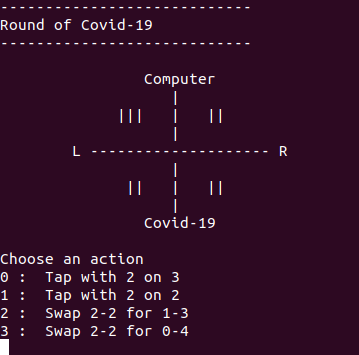
\includegraphics[scale = 0.6]{img/preview.png}
    %\caption{Caption}
    %\label{fig:my_label}
\end{figure}{}

\clearpage

\tableofcontents



%\section*{Notations}
%\label{sec:notations}

%The following variable notations will be applied in this work:

%\begin{itemize}
%    \item[--] $K$: number of latent topics considered
 %   \item[--] $D$: number of documents considered 
%    \item[--] $W$: vocabulary size 
%    \item[--] $\alpha$: parameter of the Dirichlet prior on the per-document topic distributions
%    \item[--] $\beta$: parameter of the Dirichlet prior on the per-topic word distribution
%    \item[--] $\theta_j = \{\theta_{jk}\}$: topic distribution for  document $j$, over $K$ topics
%    \item[--] $\phi_k = \{\phi_{kw}\}$: word distribution for topic $k$, over $W$ words
%    \item[--] $z_{ij}$: topic for the word i of document j
%    \item[--] $x_{ij}$: word i of document j
%    \item[--] $\vect{\theta}$: $(D\times K)$ matrix composed of rows $\theta_1, \ldots,  \theta_D$, which are distributions over topics
%    \item[--] $\vect{\phi}$: $(K\times W)$ matrix composed of rows $\phi_1, \ldots,  \phi_K$, which are distributions over words
%    \item[--] $\vect{z}$: $(W \times D)$ matrix composed of $z_{ij}$
%    \item[--] $\vect{x}$: $(W \times D)$ matrix composed of $x_{ij}$
%\end{itemize}

\clearpage

\section{Description of the game}

The following description (rules, interface) can also be found in the file $\verb|README.md|$ within the repository and in the game menu when launching the game so you might want to skip this part.

TapnSwap is a $2$-player game. Both players have a variable number of fingers on both of their hands. If one player has a hand composed of more than $4$ fingers, this hand is "killed". The goal of the game is to kill both hands of the opponent player.

\subsubsection*{First round}
\addcontentsline{toc}{subsection}{First round} 


Each player starts with $1$ finger on each hand and one of them has to make the first move. The configuration of hands is then:

\begin{verbatim}
Round of Player 1
------------------

            Player 2                
               |                    
           |   |   |                
               |                    
    L -------------------- R        
               |                    
           |   |   |                
               |                    
            Player 1 
            
\end{verbatim}

Both players are separated from each other by the horizontal line. The main vertical line separates the hands of both players (L: left hands, R: right hands). There is currently $1$ finger on each hand of each player.

\subsubsection*{Actions}
\addcontentsline{toc}{subsection}{Actions} 


At each round of the game, each player has to choose an action among the list of possible actions. There are $2$ main kinds of actions: tap and swap.

\addcontentsline{toc}{subsubsection}{Tap} 

\begin{itemize}
    \item Tap actions involve adding the number of fingers on one of your hands to one of your opponent's hands.
\end{itemize}{}

For instance, with the previous initial configuration, Player $1$ may tap only with $1$ (both of Player $1$'s hands have $1$ finger) on $1$ (both of Player $2$'s hands have $1$ finger). If it happens, the configuration of hands at the next round is then:

\begin{verbatim}
Round of Player 2
------------------

            Player 1                
               |                    
           |   |   |                
               |                    
    L -------------------- R        
               |                    
          ||   |   |                
               |                    
            Player 2                

\end{verbatim}{}

Player $2$ had $1$ finger on each hand but Player $1$ tapped with $1$ so now Player $2$ has one hand with $1+1 = 2$ fingers.

Now let's consider a more complex example:

\begin{verbatim}
Round of Player 1
------------------

            Player 2                
               |                    
          ||   |   ||||             
               |                    
    L -------------------- R        
               |                    
         |||   |   |                
               |                    
            Player 1                

\end{verbatim}{}

It is Player $1$'s round. Her hands have respectively $3$ and $1$ fingers while Player $2$ has hands with $2$ and $4$ fingers. Player $1$ can then tap with $3$ or $1$ on a hand of Player $2$, that is on $2$ or $4$.

Player $1$ is able to kill the hand of Player $2$ with $2$ fingers, by tapping with $3$ on $2$ ( $3+2 = 5 > 4$ ). The next round is then:

\begin{verbatim}
Round of Player 2
------------------

            Player 1                
               |                    
         |||   |   |                
               |                    
    L -------------------- R        
               |                    
               |   ||||             
               |                    
            Player 2                

\end{verbatim}{}

Now Player $2$ has lost a hand. Notice that Player $1$ could have killed the hand of Player $2$ which has $4$ fingers instead, in the same way.

\addcontentsline{toc}{subsubsection}{Swap} 

\begin{itemize}
    \item Swap actions consist in exchanging some fingers of one of your hand to the other one.
\end{itemize}{}

To illustrate this process, let's come back to the previous complex example:

\begin{verbatim}
Round of Player 1
------------------

            Player 2                
               |                    
          ||   |   ||||             
               |                    
    L -------------------- R        
               |                    
         |||   |   |                
               |                    
            Player 1                

\end{verbatim}{}

Instead of tapping with $1$ or $3$, Player $1$ may swap some fingers from one of her hands to the other. By swapping $1$ finger, Player $1$ can obtain the configuration of hands $2$-$2$ or $4$-$0$. Let's look at the first possibility:

\vspace{2\baselineskip}

\begin{verbatim}
Round of Player 1
------------------

            Player 2                
               |                    
          ||   |   ||||             
               |                    
    L -------------------- R        
               |                    
          ||   |   ||               
               |                    
            Player 1                

\end{verbatim}{}

By swapping, Player $1$ gets the configuration of hands $2$-$2$. Changing the hand that loses $1$ finger, Player $1$ could have obtained the configuration $4$-$0$.

There is one main restriction to swap actions: swapping to an identical but reversed configuration is NOT allowed. For instance, in this case, Player $1$ could not have swapped from $3$-$1$ to $1$-$3$, exchanging $2$ fingers.

But it is still possible to exchange $2$ fingers. For instance, a swap from $3$-$2$ to $1$-$4$ is a valid swap.

Note that it is also possible to revive a killed hand:

\begin{verbatim}
Round of Player 1
------------------

            Player 2                
               |                    
          ||   |   |                
               |                    
    L -------------------- R        
               |                    
          ||   |                    
               |                    
            Player 1                

\end{verbatim}{}

In this case, Player $1$ has one hand with $2$ fingers and a killed hand. Exchanging $1$ finger from the left to the right, Player $1$ may revive the killed hand:

\begin{verbatim}
Round of Player 1
------------------

            Player 2                
               |                    
          ||   |   |                
               |                    
    L -------------------- R        
               |                    
           |   |   |                
               |                    
            Player 1                

\end{verbatim}{}

That's all for the rules !

\section{Training}

The training of the agent is done via $Q$-learning, which is a specific kind of Reinforcement Learning algorithm. In classical Reinforcement Learning, an agent evolves in an environment in the following way: starting from an initial state $s_0$, the agent chooses an action $a_0$, the environment responds to the agent by giving its new state $s_1$ and a reward $r_0$. The same process keeps going for next time steps. At time step $t$, the agent is in state $s_t$, chooses action $a_t$ and gets its next state $s_{t+1}$ and the corresponding reward $r_t$ by the environment. 

\subsubsection*{The agent and the environment}
\addcontentsline{toc}{subsection}{The agent and the environment} 


In a $2$-player game like TapnSwap, the agent is one player that should learn the optimal policy (or strategy). The environment is the entity that is impacted by the agent's actions and that responds to the agent by giving its new states and rewards. One trivial choice for the environment is the agent's opponent.

\subsubsection*{Current state $s_t$}
\addcontentsline{toc}{subsection}{Current state $s_t$}

The current state of the agent is a list of $2$-sized lists containing the number of fingers of each hand. For instance, if the current configuration is:

\begin{verbatim}
Round of Agent
---------------

            Agent's opponent                
                   |                    
              ||   |   ||||             
                   |                    
        L -------------------- R        
                   |                    
             |||   |   |                
                   |                    
                 Agent 
\end{verbatim}

the current state of the agent is $\verb|[[3,1], [2,4]]|$. Note that the lists are firstly (agent then opponent) and secondly ordered (left hand then right hand). The initial state $s_0$ is $\verb|[[1,1], [1,1]]|$.

\subsubsection*{Action $a_t$}
\addcontentsline{toc}{subsection}{Action $a_t$}

Actions in back-end (file $\verb|tapnswap.py|$) are represented differently depending on whether they are tap or swap actions.

Tap actions are coded as $\verb|[0, tapping_hand, tapped_hand]|$ where $\verb|tapping_hand|$ is the hand of the agent involved in tap action ($0$: left hand, $1$: right hand) and $\verb|tapped_hand|$ is the hand of the agent's opponent that receives the tap action from the agent (same binary coding).

Swap actions are coded as $\verb|[1, giving_hand, exchange_nbr]|$ where $\verb|giving_hand|$ is the hand of the agent that gives some of its fingers to the other hand (same binary coding as before) and $\verb|exchange_nbr|$ is the amount of such fingers.

In file $\verb|agent.py|$, the agent initializes itself by creating an integer coding for all the actions in the previous format. At each time step, the agent gets the list of possible actions, code them in integers, chooses between them and send the decoded chosen action to back-end.

\subsubsection*{Next state $s_{t+1}$}
\addcontentsline{toc}{subsection}{Next state $s_{t+1}$}

The next state of the agent is given by the environment after that the agent chooses the action $a_t$. It is the configuration of hands obtained after the round of the agent's opponent which follows action $a_t$.

\subsubsection*{Reward $r_t$}
\addcontentsline{toc}{subsection}{Reward $r_t$}

The most difficult task in Reinforcement Learning is often determining the rewards corresponding to each transition ($s_t$, $a_t$, $s_{t+1}$). In this game, it is difficult to find such rewards without adding bias to the learning process (which may not be optimal). Indeed, the sole purpose of killing $1$ hand might not even be an optimal strategy at all ... Thus, I chose to give non-zero rewards to the agent if and only if the game came to an end (positive reward if game is won, negative reward if game is lost). 

\subsubsection*{RL}
\addcontentsline{toc}{subsection}{RL}

The agent's actions are determined by its policy $\pi$ (such that $a_t = \pi(s_t)$) which depends only on the current state. For $1$ game ending at $t = T$ and starting at state $s_0$, the goal of the agent is to maximize the following quantity w.r.t. $\pi$:

\begin{equation}
    V^\pi(s_0) = \mathbb{E} \ \bigg[\sum_{t=0}^T \ \gamma^t \ r_t \ | \ \pi, \ s_0\bigg]
\end{equation}{}

It is the expected sum of rewards the agent gets starting at $s_0$, following policy $\pi$. In this case, the expectation is on the new states $s_{t+1}$ given by the environment. The factor $\gamma$ gives the significance of first actions over last ones. The optimal policy $\pi^\star$ has value $V^\star = \underset{\pi}{\text{max}} \ V^\pi$ for all initial states.

\subsubsection*{$Q$-learning}
\addcontentsline{toc}{subsection}{$Q$-learning} 
 
The $Q$-function is defined similarly:

\begin{equation}
    Q^\pi(s_t, a_t) = \mathbb{E} \ \bigg[\sum_{t'=t}^T \ \gamma^{t'-t} \ r_{t'} \ | \ \pi, \ s_t, \ a_t\bigg]
\end{equation}{}

This algorithm approximates the optimal $Q$-function $Q^\star = \underset{\pi}{\text{max}} \ Q^\pi$. Note that the optimal policy is then given by $\pi^\star(s_t) = \underset{a \in \mathcal{A}_t}{\text{argmax}} \ Q^\star(s_t, a)$ where $\mathcal{A}_t$ is the set of possible actions at time $t$.

The main idea of $Q$-learning is to build an estimator $\hat{Q}$ of the optimal $Q$-function $Q^\star$. At the beginning, the agent is initialized with a full-zero matrix $\hat{Q}(s, a)$ for all states $s$ and all actions $a$. Note that, in our case, we are in tabular setting (the number of distinct state-action pairs can be stored in the memory of a computer) so there is no need of Deep Learning. As one can observe from the definitions of states and actions for TapnSwap, there are $5^4 - 1 = 624$ distinct states (the -$1$ is because the state $\verb|[[0,0], [0,0]]|$ is not possible) and $2^2$ (tap) $+ 2 \times 2$ (all swap actions can be described with $1$ or $2$ exchanged fingers only) $= 8$ distinct actions. Thus, the estimator $\hat{Q}$ is a matrix of size $624 \times 8$.

The training consists in the agent playing $N$ games. For each game, the agent starts at state $s_0$ and, while the game is not over, it takes action $a_t$ at state $s_t$ with $\epsilon$-greedy policy (probability $\epsilon$ of taking action randomly and $1-\epsilon$ of taking current optimal actions $\hat{\pi}^\star (s_t) = \underset{a \in \mathcal{A}_t}{\text{argmax}} \ \hat{Q}(s_t, a)$), observes next state $s_{t+1}$ and reward $r_t$. It then computes the Temporal Difference (TD($0$)):

\begin{equation}
    \delta_t = r_t + \gamma \ \underset{a \in \mathcal{A}_t}{\text{max}} \hat{Q}(s_t, a) - \hat{Q}(s_t, a_t)
\end{equation}{}

$\delta_t$ is an unbiased estimator of the Bellman error, which quantifies how far the estimator $\hat{Q}$ is from the optimal $Q$-function $Q^\star$. Thus, a simple way to minimize this error is to update the estimator $\hat{Q}$ at each time step in the following way:

\begin{equation}
    \hat{Q}(s_t, a_t) = \hat{Q}(s_t, a_t) + \alpha(s_t, a_t) \ \delta_t
\end{equation}{}

$\alpha(s_t, a_t)$ is the learning rate and should depend on the current state-action pair. $Q$-learning converges a.s. to the optimal $Q$-function if all state-action pairs are tried infinitely often with the learning rate satisfying Robbins-Monro conditions: I chose in this case $\alpha(s_t, a_t) = \frac{1}{\#(s_t, a_t)}$ where $\#(s_t, a_t)$ is the number of visits of the state-action pair ($s_t$, $a_t$) from the agent. The decisions of the agent and the updates of the estimator $\hat{Q}$ are coded in file $\verb|agent.py|$.

The whole process is repeated until the game is over, and for $N$ games. At the end, the near-optimal policy is $\hat{\pi}^\star(s_t) = \underset{a \in \mathcal{A}_t}{\text{argmax}} \ \hat{Q}(s_t, a)$.

An agent is thus fully determined by the pair ($\epsilon$, $\gamma$) used during training. Note that $\epsilon$ controls the trade-off between exploitation and exploration. 

\subsubsection*{The agent's opponent}
\addcontentsline{toc}{subsection}{The agent's opponent}

The opponent is a significant feature for training as it is the environment in which the agent evolves. In file $\verb|train.py|$, I implemented $2$ different ways of training for an agent: playing against a fully Random Agent or playing against another version of itself. 

Note that usually, $Q$-learning is an off-policy method, meaning that the agent should adopt an $\epsilon = 1$-greedy policy. However, firstly because of flexibility and secondly because of the influence of $\epsilon$ on the environment (when an agent plays against another version of itself), I chose to allow training for any value of $\epsilon$.

\subsubsection*{Training in practice}
\addcontentsline{toc}{subsection}{Training in practice}

In file $\verb|train.py|$, I implemented a training function that allows to train any agent (determined by $\epsilon$ and $\gamma$) during the number of games (or epochs) you want, either vsRandom (fully Random Agent opponent) or vsSelf (playing against another version of itself). At the end of training, the function saves the learned $Q$-function in a CSV format located at $\verb|Models/filename.csv|$. The typo for $\verb|filename|$ I used can be illustrated with an example: the file $\verb|Models/greedy_0_1_vsRandom.csv|$ stores the $Q$-function of an agent with $\epsilon = 0.1$ training against a Random Agent while the file $\verb|Models/greedy_0_4_vsSelf.csv|$ stores the $Q$-function of an agent with $\epsilon = 0.4$ training against another version of itself. 

Note that $\gamma$ is not specified in the name of the CSV file because it is not a relevant parameter in our case. Indeed, since the only reward is at the end of the game, there is no need to weight some rewards compared to others.

The previous training function also stores the counter of state-action pairs encountered by an agent during training. For the latter example, the counter is stored at $\verb|Models/data/count_greedy_0_4_vsSelf.csv|$.

Thus, I allowed the possibility of training an already trained model, importing the learned $Q$-function and the counter of encountered state-action pairs. It is also possible for the user to play on the shell with the learning agent DURING training as often as you want. In the same way, I allowed for a learning agent the possibility to play any number of games (without training on those) against a fully Random Agent during training, as a kind of evaluation of current training.

\section{Optimizer}

The module Optimizer found in file $\verb|validation.py|$ is used as validation step for training agents via $Q$-learning. Training can be done for many values of $\epsilon$ and for different opponents (Random Agent, Self and all sequences using those two). Indeed, it is possible to initialize the optimizer by setting $\verb|change_opp = True|$, meaning that after $1$ session of training of any agent vsRandom or vsSelf, the agents change their type of opponent for the following session of training. In this way, it is possible to alternate the $2$ types of opponents during the whole training. For instance, an agent initialized with $\epsilon = 0.1$ firstly trained vsRandom, then vsSelf, stores its learned $Q$-function in $\verb|Models/greedy_0_1_vsRandomvsSelf.csv|$.

\subsubsection*{Method \ $\mathtt{grid\_search}$}
\addcontentsline{toc}{subsection}{Method \ $\mathtt{grid\_search}$}

The method $\verb|grid_search|$ of module Optimizer computes the fraction of an agent's wins over a given number of games against a Random Agent. This fraction is computed as a function of the number of games used for training the agent. It then provides a way of visualizing the progress made by all trained agents (different values of $\epsilon$ and different opponents). 

For instance, Figure~\ref{fig:training} depicts what you can get by training an agent with $\epsilon = 0.8$ vsSelf during $100$ games.

\begin{figure}[h]
    \centering
    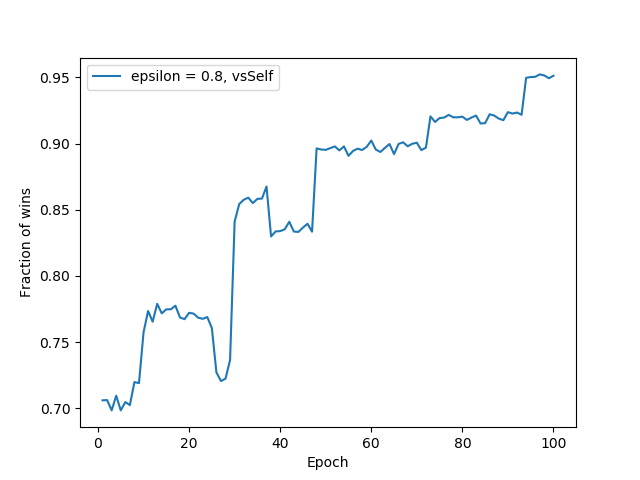
\includegraphics[scale = 0.8]{img/training.png}
    \caption{Performance of an agent initialized with $\epsilon = 0.8$ and trained vsSelf (another version of itself) during training. On the $y$-axis is represented the fraction of wins the agent has got when playing $10000$ games against a Random Agent.}
    \label{fig:training}
\end{figure}{}

At each epoch, the training agent has played $10000$ games against a Random Agent and the fraction of wins is represented on the $y$-axis. One can observe that the agent reaches local maxima (different branch - perhaps still a good strategy - than the optimal policy) which may last $20$ epochs forming a \textit{plateau}, then performs worse followed by a great progress. Note that at each time that an agent is tested (here and in what follows), it chooses its actions with its version of optimal policy (that is $\epsilon = 0$) so that the parameter $\epsilon$ is only significant during training.

Those testing results obtained during training are stored in a txt file. For the previous example, the results of training are stored in $\verb|Models/train/GS_epsilon_0_8_vsSelf.txt|$. In those txt files, each line corresponds to an epoch result in the format: epoch, score of training agent, number of finished games, number of played games. Note that, if the new trained agent loses against its old version (before the training), the method $\verb|grid_search|$ cancels the training and keeps the past version of the training agent. This may be useful in case of several sessions of training.
      
At the end of all trainings, the method $\verb|grid_search|$ simulates a tournament between all trained agents. Each agent plays $10$ games against all others and the scores of each model against another 
are stored in a CSV file located at $\verb|Models/results/tournamentK.csv|$ where $K$ is the number of tournaments the module Optimizer has simulated. A txt file is also generated using the previous CSV file: it displays rankings of each model, alongside its total score against all other models. Those files are located at $\verb|Models/results/tournamentK.txt|$.

The method $\verb|grid_search|$ has an option $\verb|retrain|$ which, if set to True, does the previous process for already trained models. If the option $\verb|change_opp|$ is also set to True at the initialization of the module Optimizer, the already trained agents are retrained normally (first output) and retrained with a different opponent than before (second output) which may be useful to compare agents among which some alternate the type of their opponent. In this way, if you want to compare trained agents among which some alternate their type of opponent, it is necessary to initialize the Optimizer with $\verb|change_opp = True|$ and then firstly run the method $\verb|grid_search|$ with $\verb|retrain = False|$ (no model already trained for now) and secondly to run it another time but with $\verb|retrain = True|$. 

\subsubsection*{Method \ $\mathtt{retrain\_best\_models}$}
\addcontentsline{toc}{subsection}{Method \ $\mathtt{retrain\_best\_models}$}

Looking at the results of the tournaments output by the $\verb|grid_search|$ method, it is then possible to retrain some of the trained agents, according to their total score during the previous tournament.

The method $\verb|retrain_best_models|$ looks at the previous tournament ranking txt file and selects some of the best current models according to their total score. The selection is made by keeping the models that have a total score above a given fraction of the best total score.

It is worth noting that the values of $\epsilon$ not represented by the corresponding selected best models are definitely discarded by the Optimizer. Once selected, those models are retrained for a given number of epochs, without playing against a Random Agent during training (as opposed to $\verb|grid_search|$ method), and eventually participate to a tournament, in the same way than before. Note that only the values of $\epsilon$ matter in the participation of agents in the next tournament and not their type of opponent. For instance, if an agent with $\epsilon = 0.1$ previously trained vsRandom has performed very poorly in the previous tournament while, with the same value of $\epsilon$ but trained vsSelf, it has performed very well, both agents will participate to the tournament output by this method (but only the good one will have been retrained before the tournament).

Since the input and the ouput of $\verb|retrain_best_models|$ are both a tournament ranking txt file, it is possible to run several times this method, each time decreasing the number of selected agents, until you get the number of well-performing agents you want. Note that, because of the input to the $\verb|retrain_best_models|$ method, it is necessary to run the $\verb|grid_search|$ method before, at least once.

\section{Experiments}

Given the modules and functions defined above, this is what I have achieved to study the possible strategies of the game.

\subsubsection*{Implementation}
\addcontentsline{toc}{subsection}{Implementation}

In the implementation provided by this repo, I have initialized the module Optimizer with $\verb|change_opp = True|$, meaning that each time that agents are retrained with the $\verb|grid_search|$ method the agents both keep their previous type of opponent and alternate them (leading to $2$ more agents output than for $\verb|change_opp = False|$). The values of $\epsilon$ that I considered were $0.1$, $0.2$, $\dotsc$, $0.9$, $1.0$. The value $\epsilon = 0$ is not really interesting, especially if the agent is trained vsSelf which leads to a null exploration.

Then, I have runned the method $\verb|grid_search|$, training the agents initialized with the previous values of $\epsilon$ vsRandom and vsSelf for $5000$ epochs, testing them each $1000$ epochs with $10000$ games against a Random Agent. I have re-runned this method with $\verb|retrain = True|$ with the same previous parameters, meaning that I trained the agents normally (for $10000$ epochs from the very start) and also changing their opponents (for instance, $5000$ epochs vsRandom and then $5000$ epochs vsSelf). This allowed me to train agents for all of the previous values of $\epsilon$ vsRandom, vsSelf, vsRandomvsSelf and vsSelfvsRandom, each of them with a total number of training epochs equal to $10000$. At the end, the method creates a tournament ($\verb|Models/results/tournament2.txt|$ in this repo) which compares all of current agents. The resulting rankings are strongly stochastic and depend a lot on the chance of having exploring and exploiting enough the trained agents got. This is not a problem since the purpose here is to approach the optimal policy as soon as possible.

After having trained the agents with $4$ combinations of opponents (vsRandom, vsSelf, vsRandomvsSelf, vsSelfvsRandom) for $10000$ epochs, I have runned the method $\verb|retrain_best_models|$ keeping all agents with a total score above $30$\% of the max total score in the previous tournament ($\verb|Models/results/tournament2.txt|$ in this repo) and training them for $40000$ more epochs. The output is the file $\verb|Models/results/tournament3.txt|$. 

Finally, I have runned this method $4$ more times, each time training the best models during $50000$ epochs and reducing the number of best models kept. The last output in this repo is $\verb|Models/results/tournament7.txt|$. In order to look for the optimal policy, I kept going on my local machine but the total scores of the top $3$ best models did not change so I decided to stop. Indeed, playing against the best models at this time showed me that it was enough.

\subsubsection*{Results}
\addcontentsline{toc}{subsection}{Results}

In fact, when playing against the previous best agents, I was not able to win if I was the player to make the first move. I think I have tried all possibilities when playing against my top agent (which I chose to be the difficult level on the game menu), without being able to win a single time (if I was the player to make the first move).

This project showed me that this game can be 'cracked', meaning that \textbf{there exists a strategy you could always win with, if you don't start}. This was one of my main interrogation about this game and, before this implementation, I was pretty close to the optimal policy since I have played this game a lot. For the sole purpose of discovering this strategy, this project was worth it.

As a consequence, if you let the trained agent start and that you apply the optimal policy, you are sure to win, meaning that all depends on who starts. However, this has led to an unforeseen negative point: in practice, all good performing agents were trained against another version of themselves (vsSelf) at some point (which is not surprising once the exploration is in the good direction) so that, without having found the full optimal policy (meaning that you always win in any configuration), they were able to win if they did not start. Thus, the trained agents that started during the training were sure to lose and did not explore other configurations than the ones explored in their current optimal policy. That's why it may be possible to win if you let the trained agent start, without applying the optimal policy (but not so easy !).

A way of improvement that I did not try is to forbid the optimal strategy (at some point or at the last move) to train agents in other configurations than the ones encountered in the optimal policy.


\end{document}